\documentclass[../main.tex]{subfiles}
\graphicspath{{\subfix{../images/}}}

\begin{document}
% Provide an overview on how the user interface(s) of your system will look like; if you have included this part in the RASD, you can simply refer to what you have already done, possibly providing here some extensions if applicable


\subsection{Mockups}

\begin{figure}[!htb]
  \centering
  \begin{minipage}[b]{0.3\textwidth}
    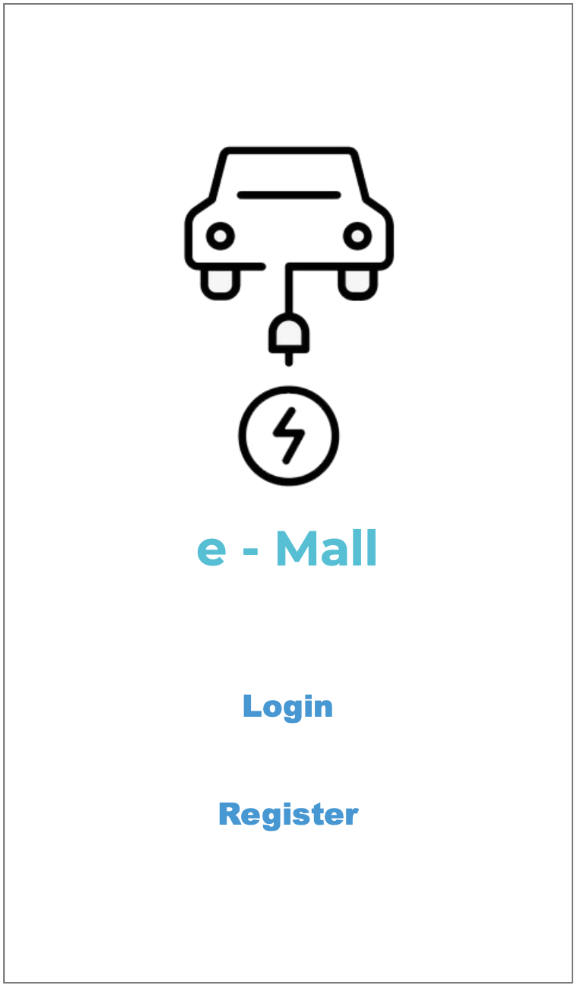
\includegraphics[width=35mm]{Mockups/mk_mainpage.png}
    \caption{Login page}
    \label{mk:mainpage}
  \end{minipage}
  \hfill
  \begin{minipage}[b]{0.3\textwidth}
    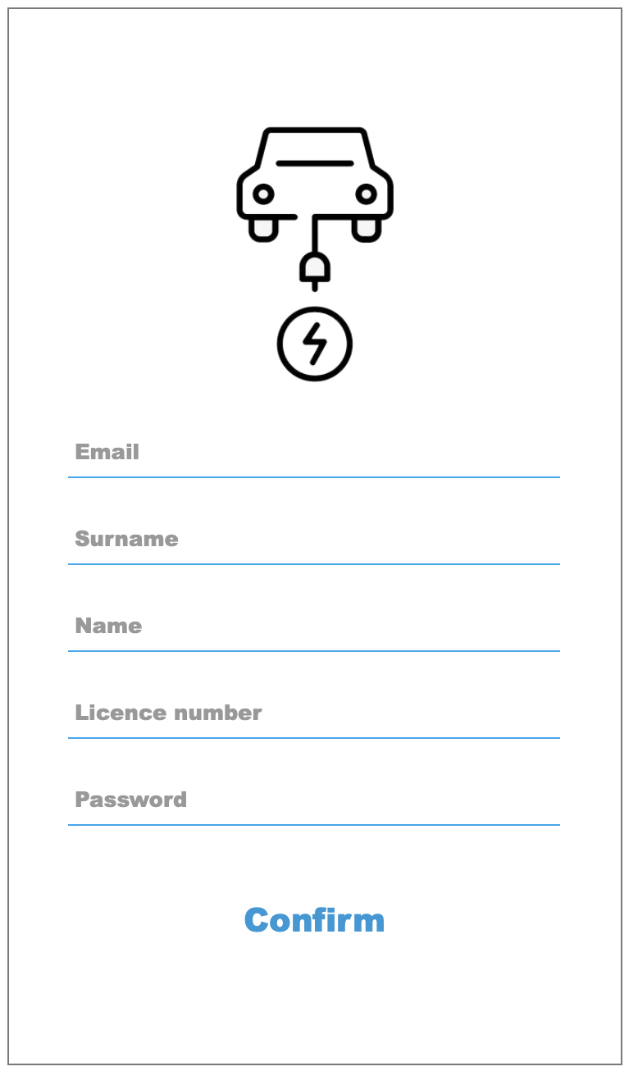
\includegraphics[width=35mm]{Mockups/mk_signuppage.png}
    \caption{Registration Form}
    \label{mk:signup}
  \end{minipage}
\end{figure}


\begin{figure}[!htb]
  \centering
  \begin{minipage}[b]{0.3\textwidth}
    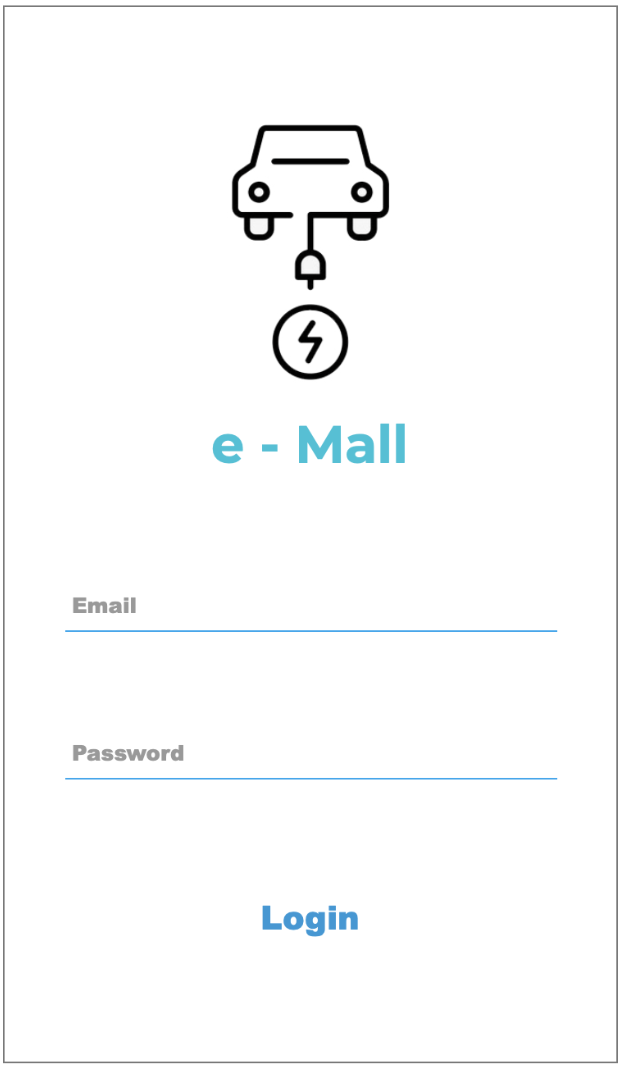
\includegraphics[width=35mm]{Mockups/mk_loginpage.png}
    \caption{Login Form}
    \label{mk:login}
  \end{minipage}
\end{figure}
\noindent
The Login Page (Figure.\ref{mk:mainpage}) and the Login Form (Figure.\ref{mk:login}) are shared for both type of users (Driver and Operator), while the Registration Form (Figure.\ref{mk:signup}) allows a driver to register an account without privileged functionalities. 
\clearpage
\newpage


\subsubsection{Driver's UI}
\begin{figure}[!htb]
  \centering
  \begin{minipage}[b]{\textwidth}
  \centering
    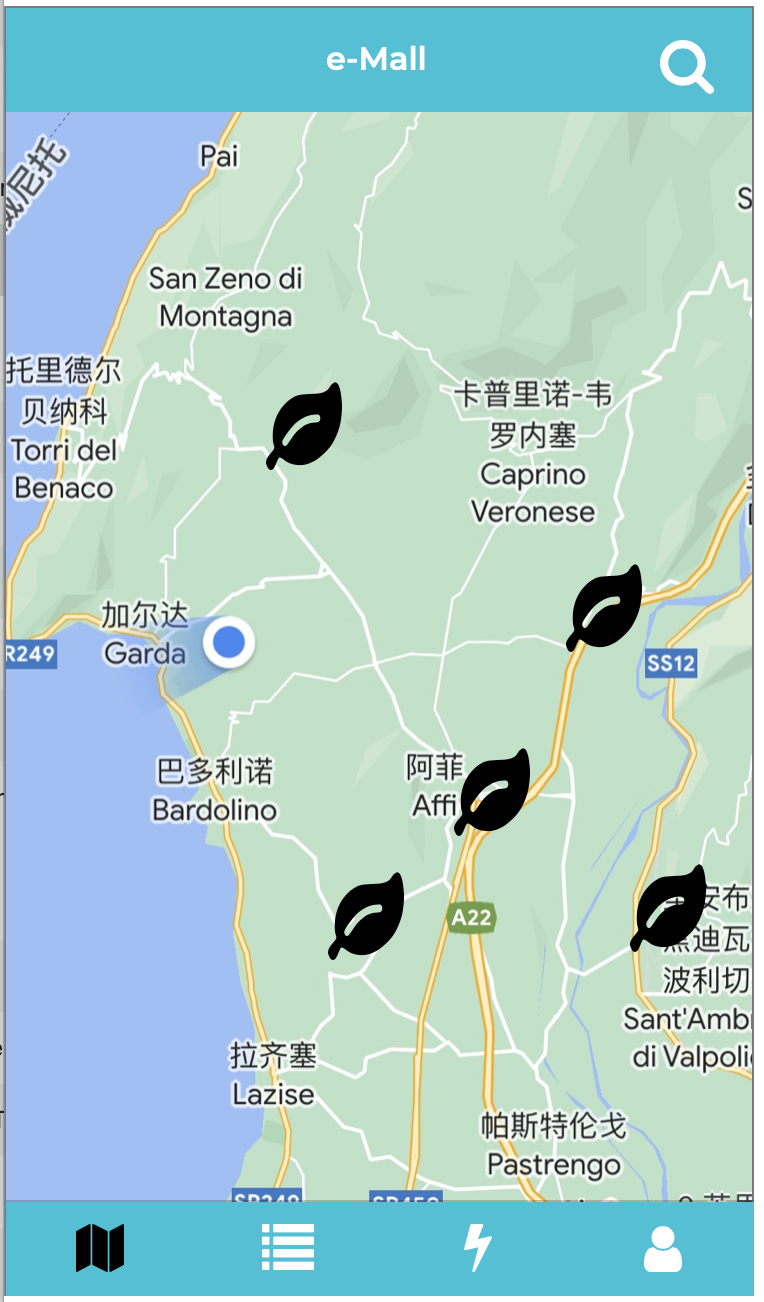
\includegraphics[width=35mm]{Mockups/mk_dv_map.png}
    \caption{Map Page}
    \label{fig:class}
  \end{minipage}
\end{figure}
\\
\noindent
This represents the Main Page for the driver, as he is redirected here after the login operation. There is a map showing the position of the Driver and the nearby charging stations, which are represented with their icon (leaves in this case), where the Driver can select one of those to see further information. The search icon above is used for searching nearby charging stations according to the inserted address. 
\begin{figure}[!htb]
    \centering
  \begin{minipage}[b]{\textwidth}
  \centering
    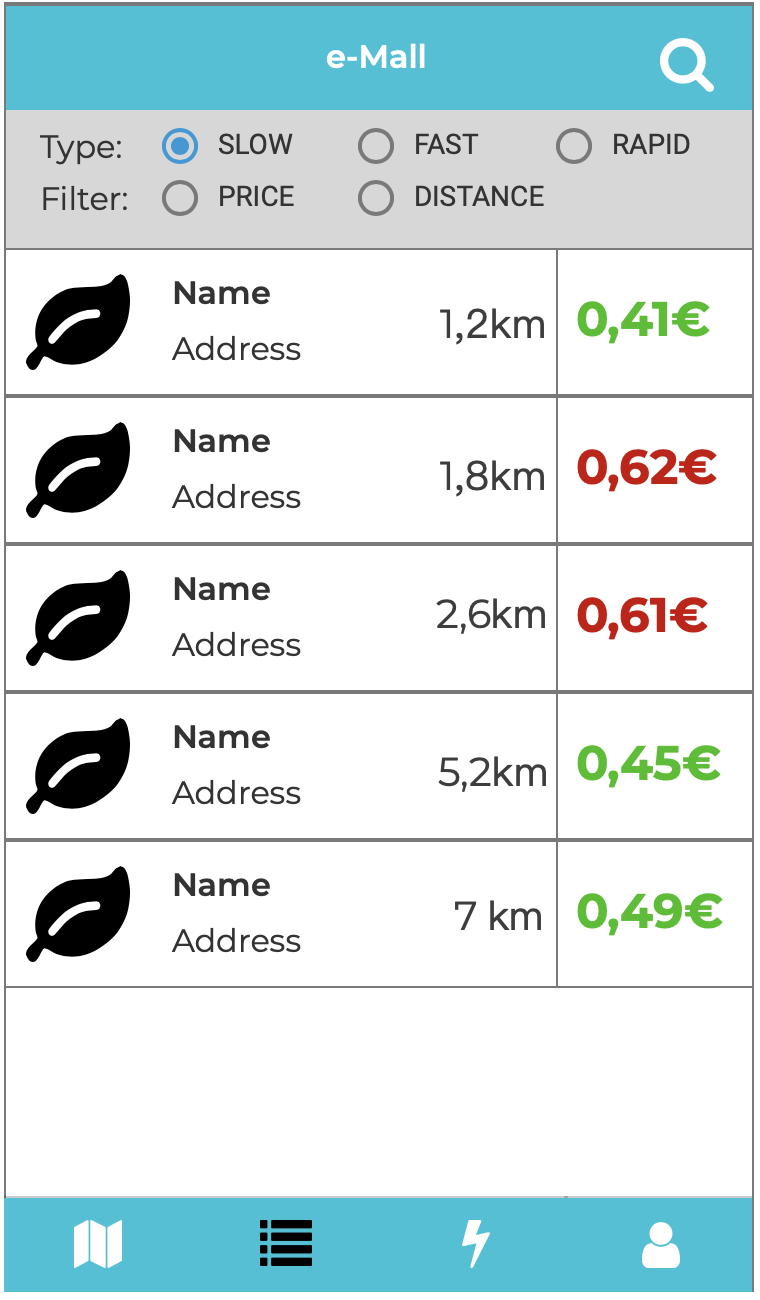
\includegraphics[width=35mm]{Mockups/mk_dv_list.png}
    \caption{List Page}
    \label{fig:class}
  \end{minipage}
\end{figure}\\
There is a list of charging stations where the user can filter selecting the buttons on top of the application. Driver can select one of those to see further information.
\newpage
\begin{figure}[!htb]
  \centering
  \begin{minipage}[b]{\textwidth}
    \centering
    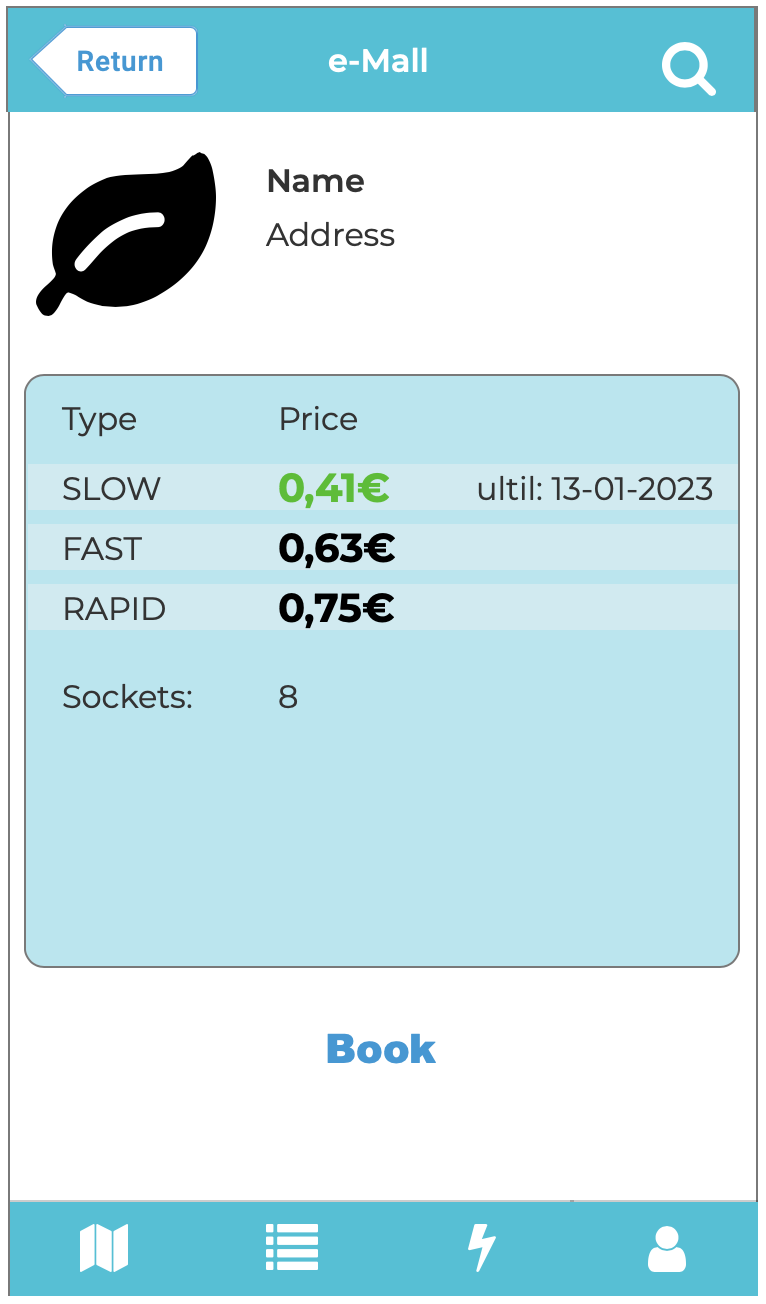
\includegraphics[width=35mm]{Mockups/mk_dv_csinfo.png}
    \caption{Charging Station Info}
    \label{fig:class}
  \end{minipage}
  \end{figure}\\
  \noindent
The page is showing information on the charging station. In this page Driver can book a charge.
  \begin{figure}[!htb]
  \centering
  \begin{minipage}[b]{\textwidth}
    \centering
    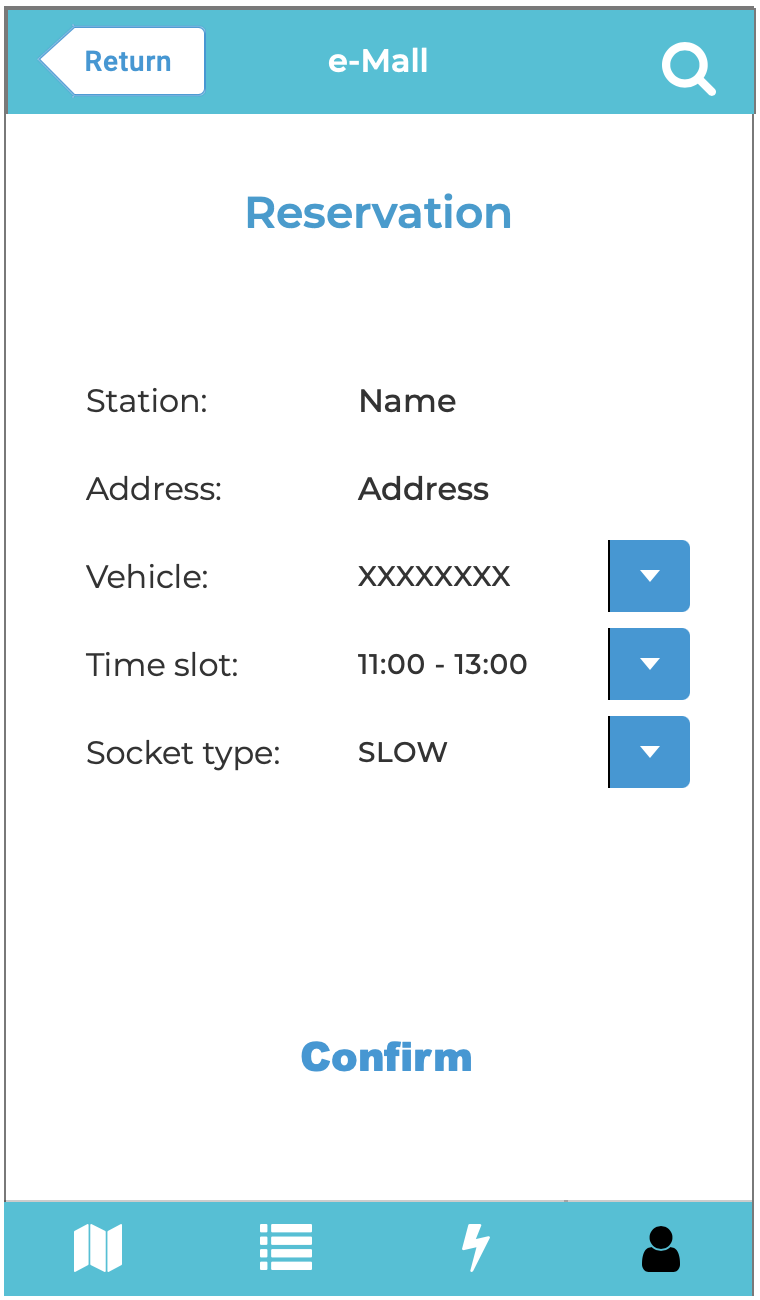
\includegraphics[width=35mm]{Mockups/mk_dv_book.png}
    \caption{Reservation Page}
    \label{fig:class}
  \end{minipage}
\end{figure}\\
In this page, Driver can compile the forum and click on confirm button to complete the booking process.
\newpage

\begin{figure}[!htb]
  \centering
  \begin{minipage}[b]{\textwidth}
  \centering
    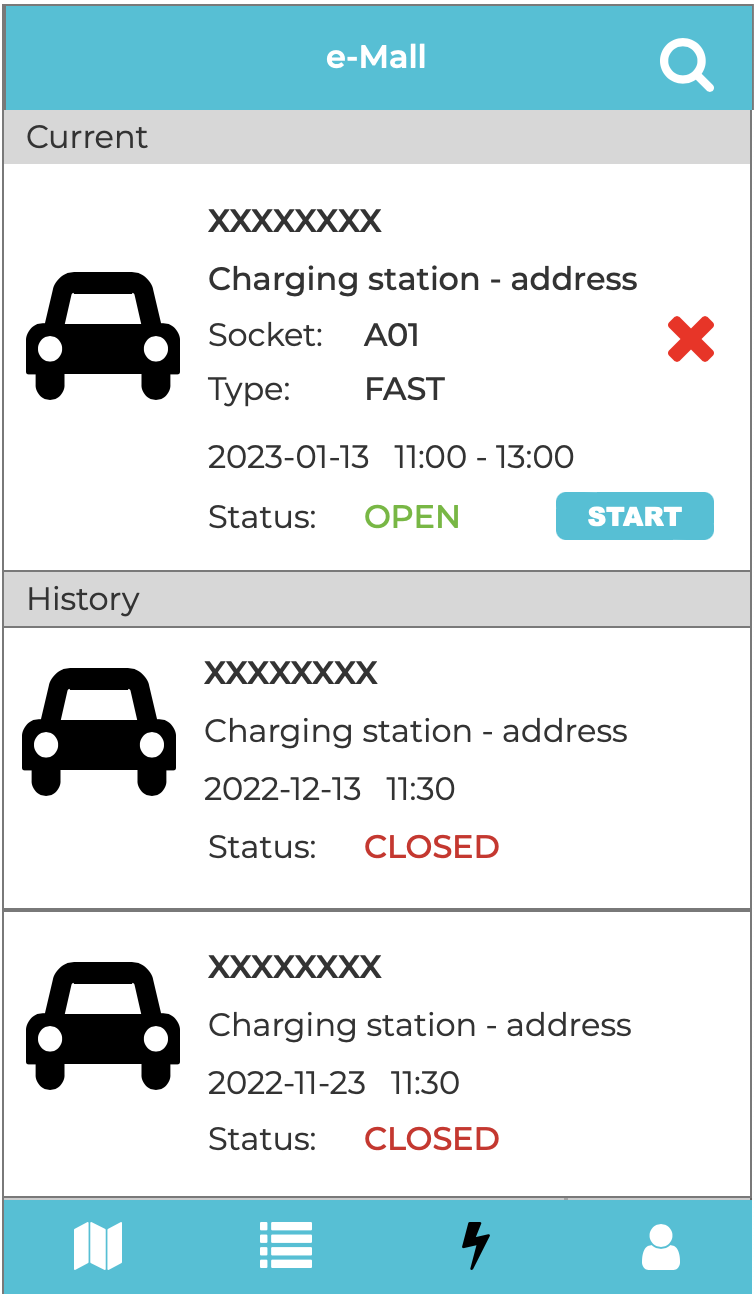
\includegraphics[width=35mm]{Mockups/mk_dv_reservs.png}
    \caption{List of reservations}
    \label{fig:class}
  \end{minipage}
  \hfill
  \end{figure}
  \noindent
There is the list containing the current and past reservations. Under “current” it appears the last reservation that hasn’t completed yet, where the user is able to cancel it or start charging his vehicle when he arrived at the charging station.
  \begin{figure}[!htb]
\centering
  \begin{minipage}[b]{\textwidth}
  \centering
    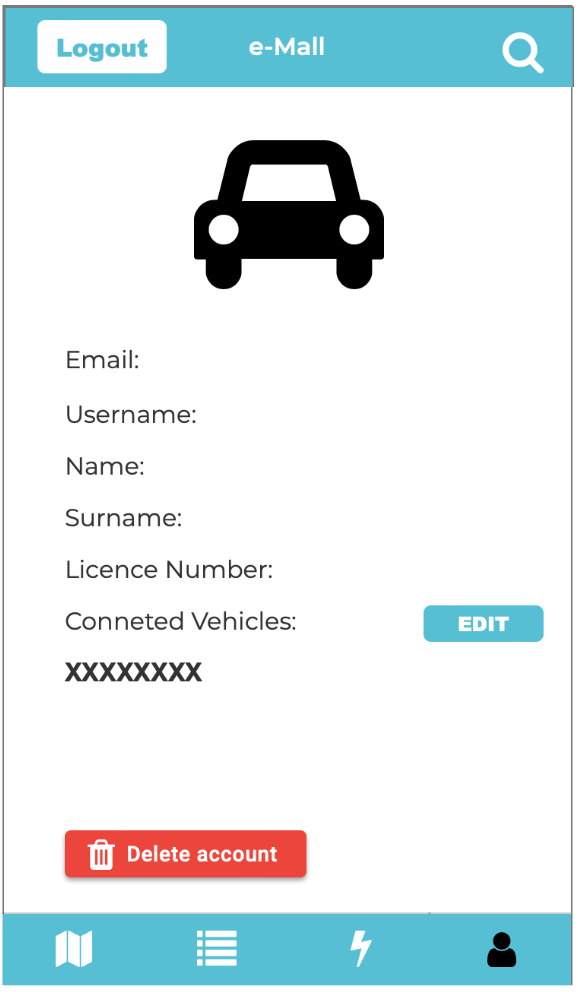
\includegraphics[width=35mm]{Mockups/mk_dv_info.png}
    \caption{Account page}
    \label{fig:class}
  \end{minipage}
\end{figure}\\
Here, all the Driver's profile information is reported. He can edit the list of vehicles he is connected to, and he can choose to delete his own account. 
\clearpage
\newpage

\subsubsection{Operator's UI}
\begin{figure}[!htb]
  \centering
  \begin{minipage}[b]{\textwidth}
  \centering
    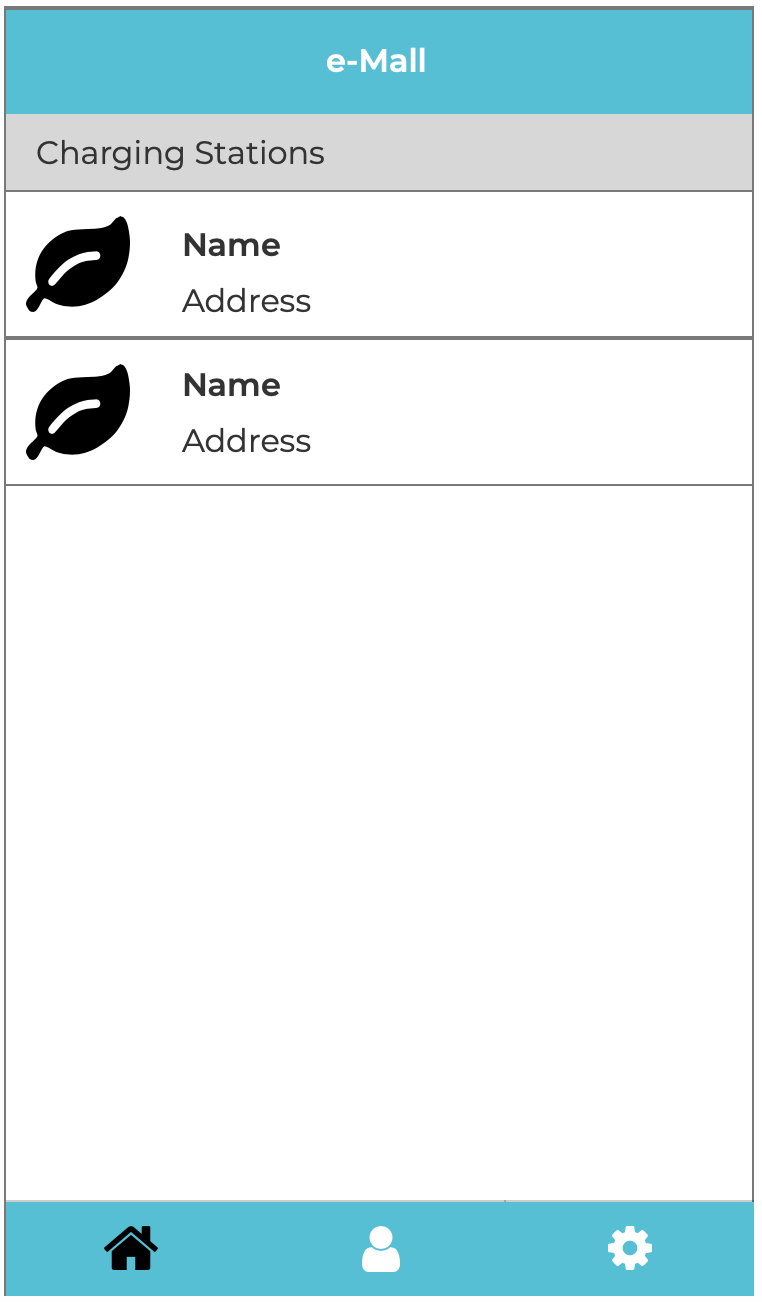
\includegraphics[width=35mm]{Mockups/mk_op_listcss.png}
    \caption{List of Charging Stations}
    \label{fig:class}
  \end{minipage}
  \hfill
  \end{figure}
  \noindent
This is the Main Page for the logged Operator. It shows the list of Charging stations that the current Operator can manage.

  \begin{figure}[!htb]
  \centering
  \begin{minipage}[b]{\textwidth}
    \centering
    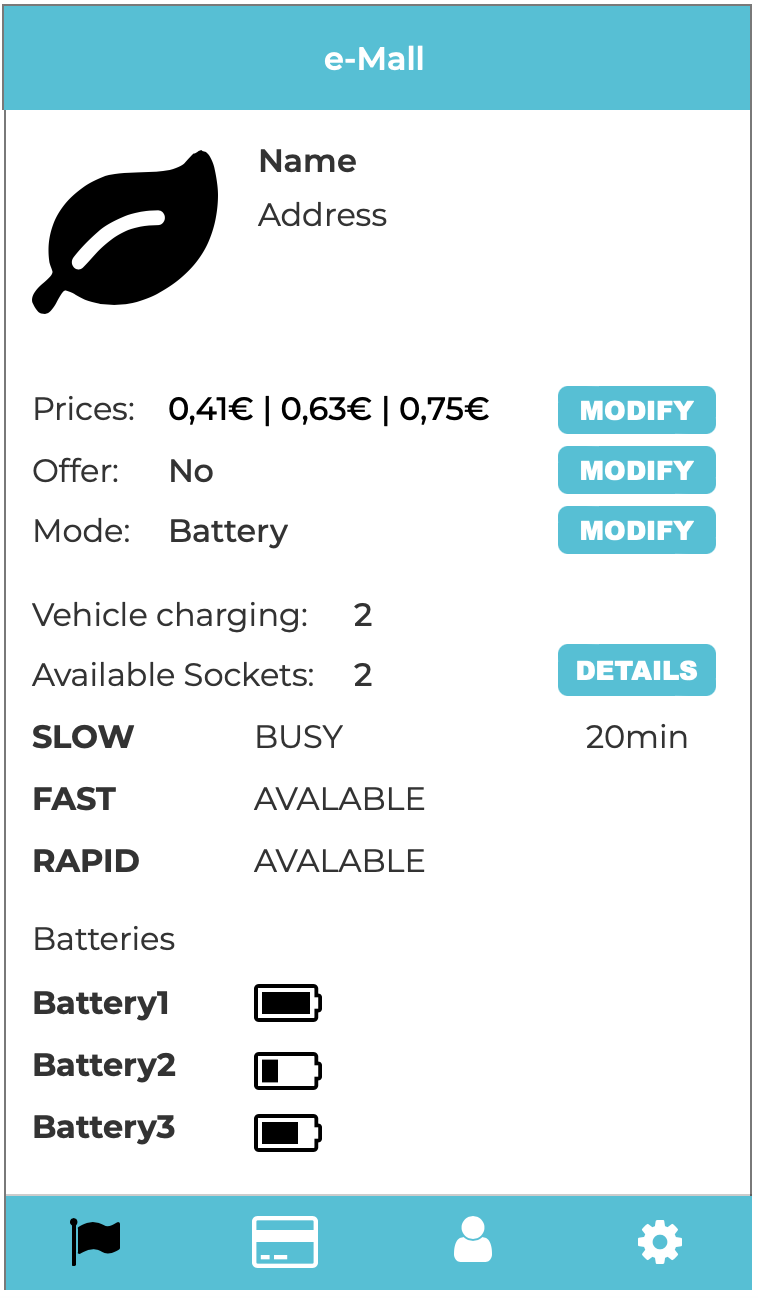
\includegraphics[width=35mm]{Mockups/mk_op_csinfo.png}
    \caption{Charging Station Info}
    \label{mk:opcs}
  \end{minipage}
\end{figure}\\
Information on the selected charging station. The Operator can edit some fields and see more details about them.
\newpage


\begin{figure}[!htb]
  \centering
  \begin{minipage}[b]{\textwidth}
  \centering
    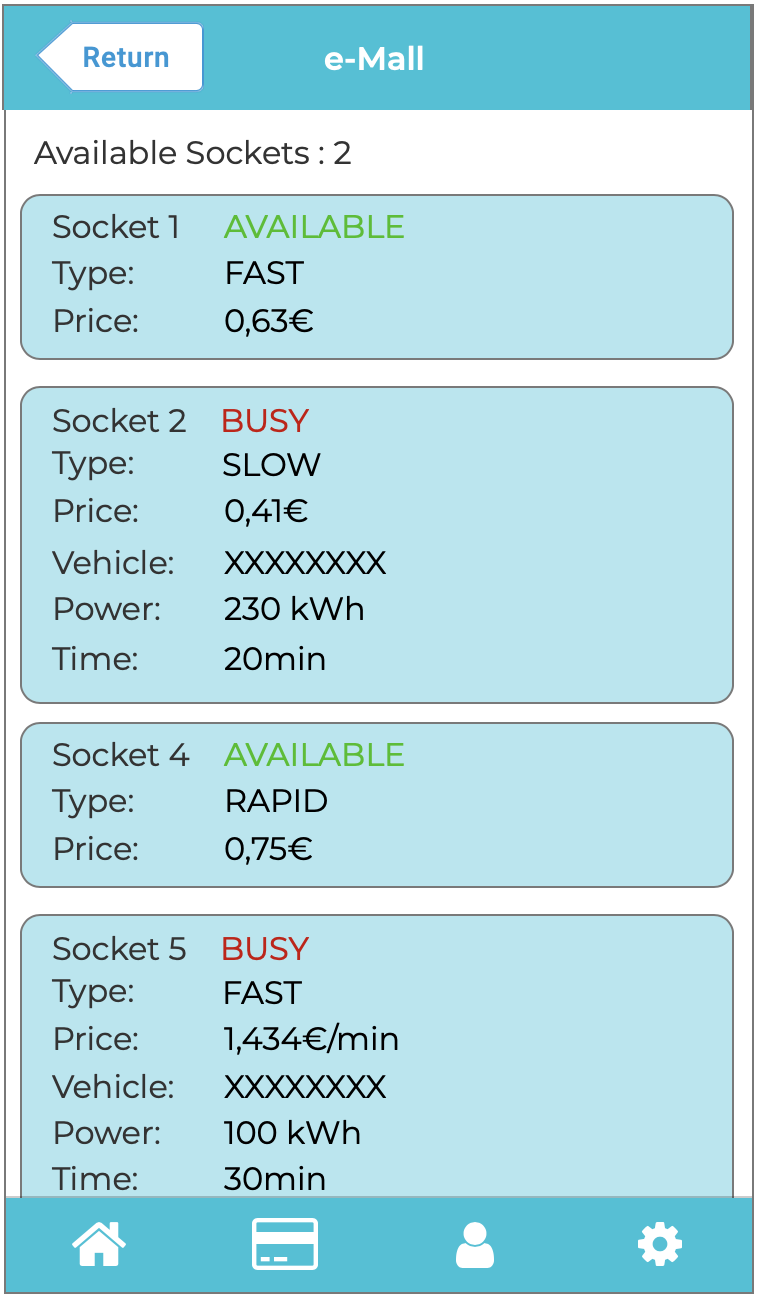
\includegraphics[width=35mm]{Mockups/mk_op_socketinfo.png}
    \caption{Sockets Info}
    \label{fig:class}
  \end{minipage}
  \hfill
\end{figure}
\noindent
In this page, there is more information on the charging station: details on each socket such as its status, price, charging vehicle, power absorbed by vehicle and the time left to complete the charging process.

  \begin{figure}[!htb]
  \centering
  \begin{minipage}[b]{\textwidth}
  \centering
    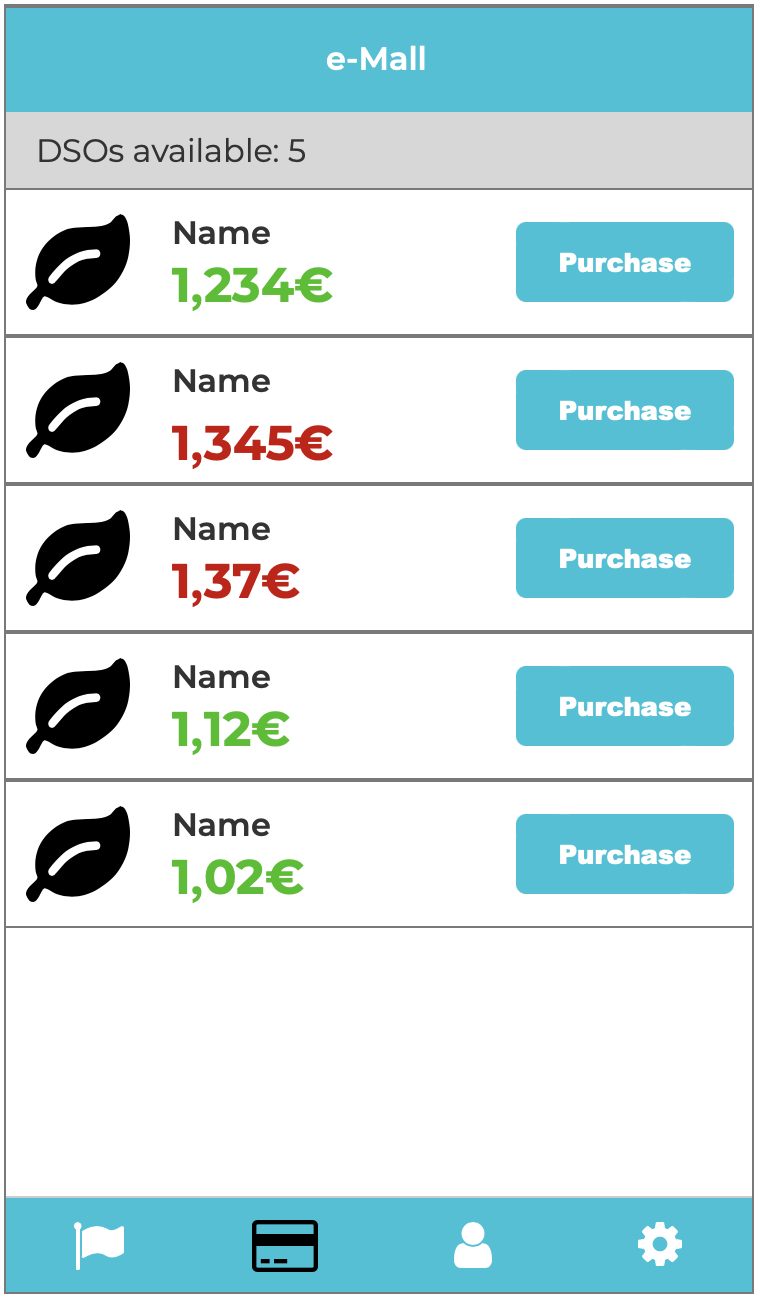
\includegraphics[width=35mm]{Mockups/mk_op_dsos.png}
    \caption{List of DSOs}
    \label{fig:class}
  \end{minipage}
\end{figure}\\
List of purchasable DSOs' energy, where Operator can acquire energy from the available DSOs.
\newpage


\begin{figure}[!htb]
  \centering
  \begin{minipage}[b]{0.3\textwidth}
  \centering
    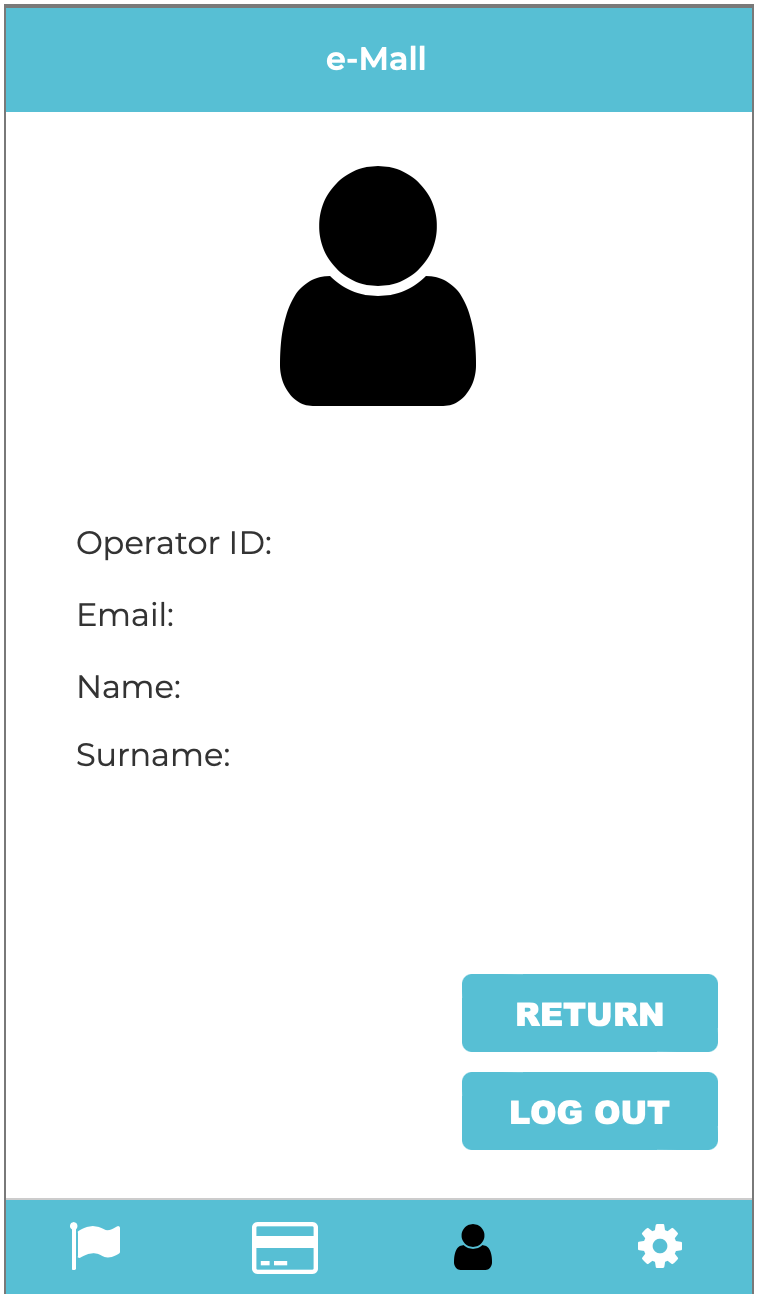
\includegraphics[width=30mm]{Mockups/mk_op_info.png}
    \caption{Account page}
    \label{fig:class}
  \end{minipage}
\end{figure}
\noindent
This is the profile of the Operator. The "Return" button lets him to return to the page where he can select the available charging stations (Figure.\ref{mk:opcs}).
\clearpage
\newpage

\end{document}